%Created on: July 8, 2014       Edited by: Wesley Kyle
%Edited on:                     Edited by:
%Edited on:                     Edited by:
%Edited on:                     Edited by:
%Edited on:                     Edited by:
%Edited on:                     Edited by:
%Edited on:                     Edited by:
%Edited on:                     Edited by:


% This is a template for the production of all future lab documents
% 
% IMPORTANT: Edit only between the line "%%%start %%% DO NOT REMOVE THIS LINE"
% and %%%end %%% DO NOT REMOVE THIS LINE
%
% To compile the tex file use the command pdflatex

\documentclass[justified]{tufte-book}
\usepackage{graphicx} % allow embedded images
\setkeys{Gin}{width=\linewidth,totalheight=\textheight,keepaspectratio}
\usepackage{amsmath}  % extended mathematics
\usepackage{booktabs} % book-quality tables
\usepackage{units}    % non-stacked fractions and better unit spacing
\usepackage{multicol} % multiple column layout facilities
\usepackage{fancyvrb} % extended verbatim environments
\fvset{fontsize=\normalsize}% default font size for fancy-verbatim environments
\usepackage{tikz} %for drawing nice pictures
\usepackage{indentfirst}
\usepackage{enumitem}
\usepackage{fancyhdr}
\usepackage{soul}
\usepackage{marvosym}
\pagestyle{fancy}
\usepackage{float}
\allowdisplaybreaks % allows equations to span two pages if needed
\restylefloat{table}
\usetikzlibrary{arrows,snakes,shapes,calc,patterns}
\usetikzlibrary{circuits.ee.IEC}
%\usepackage[T1]{fontenc}
%\usepackage[utf8]{inputenc}

\fancyhf{} % clear all header and footer fields
\fancyfoot[C]{\footnotesize \thepage}
\renewcommand{\headrulewidth}{0pt}
\renewcommand{\footrulewidth}{0pt}


\begin{document}

\chapter{X-Ray Diffraction - Companion Guide}


%%%start %%% DO NOT REMOVE THIS LINE

\section{Equipment}

% first column
\begin{minipage}[t]{0.5\textwidth}
\begin{itemize}[noitemsep]
\item Tel-X-ometer x-ray spectrometer
\item LiF crystal diffraction grating
\item Geiger counter detector
\item 1mm and 3mm lead collimator slides
\end{itemize}
\end{minipage}
%second column
\begin{minipage}[t]{0.5\textwidth}
\begin{itemize}[noitemsep]
\item Tel-Atomic Digicounter digital pulse counter
\item X-ray tube current monitoring cable
\item Fluke multimeter
\item Acrylic plastic x-ray attenuator slide plate
\end{itemize}
\end{minipage}

\section{Setup}
\begin{figure}
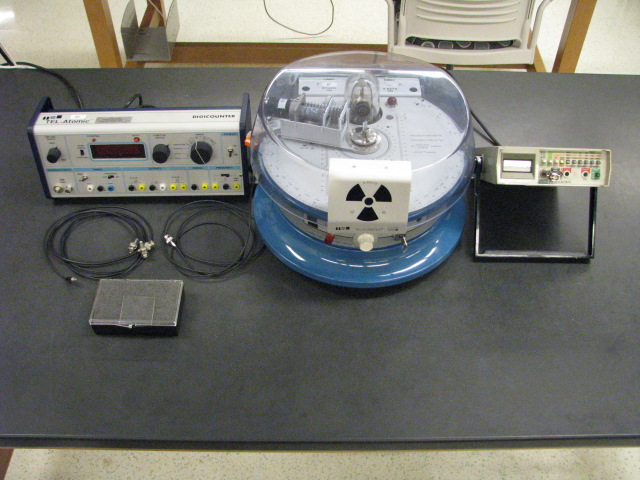
\includegraphics{X-Ray-Diffraction-Setup.jpg}
\caption{Equipment Setup}
\label{pic:XRsetup}
\end{figure}

Set up bench as shown in Figure \ref{pic:XRsetup}.

\section{Maintenance}

\begin{enumerate}
\item 
\item 
\end{enumerate}

\section{Critical Points of Failure}

There are currently no known critical points of failure.

\section{Notes to the Instructor}
\begin{enumerate}
\item It is practical to take standard single-degree steps when measuring the bremsstrahlung continuum however it is recommended that students take smaller, half-degree steps around the characteristic peaks to improve the resolution of their spectra.
\end{enumerate}

\section{Prelab Questions}
\begin{enumerate}

\item {\bf The x-ray region of the electromagnetic spectrum extends between the frequencies of $10^{17}$ Hz and $10^{20}$ Hz. For x-rays of these two frequencies, calculate the corresponding wavelength in nanometers and the corresponding energy in keV.}\newline

We know that $c=\lambda\nu$ and that E=h$\nu$. Using these relationships we can find that $10^{17}$ Hz=$3$ nm=$0.4136$ keV and $10^{20}$ Hz=$0.003$ nm=$413.6$ keV.

\item {\bf Find the energy, in keV, of an electron accelerated across a 30kV potential difference. What is the cut-off energy, in keV, of a 30kV x-ray tube?}\newline

1 keV is the energy gained by a single electron crossing a potential difference of 1 V. In this case, the electron will gain 30 keV of energy. If we have a 30 keV x-ray tube, we should see no photons possessing higher energy than 30 keV, thus 30 keV would be the cut-off energy.

\item {\bf In Figure 4, explain whether it is the left side or the right side of the x-ray spectrum that is the high energy side.}\newline

Using the following relationship,

\begin{equation}
n\lambda=2dsin\theta
\label{equ:twcg1}
\end{equation}

We can see that $\lambda$ is maximal when $\theta=90^{\circ}$ and minimal when $\theta=0^{\circ}$. This means that the left side of the plot, i.e., the smaller angles, correspond to shorter wavelengths and higher energies and the right side of the plot, i.e., the larger angles, correspond to longer wavelengths and lower energies.

\item {\bf Look up the atomic masses of lithium and fluorine, and the density of LiF. Using these values calculate the atomic spacing of LiF.}\newline

A$_{Li}$=6.94 g mol$^{-1}$ and A$_{F}$=19.0 g mol$^{-1}$ so A$_{LiF}$=25.94 g mol$^{-1}$. The density of LiF, $\rho$, is 2.64 g cm$^{-3}$. We use the following relation to find the interatomic spacing of LiF,

\begin{equation}
d=\sqrt[3]{\dfrac{A_{LiF}}{2N_A\rho}}=\sqrt[3]{\dfrac{25.94}{2(6.022\times10^{23})(2.64)}}=0.2013nm
\label{equ:twcg2}
\end{equation}

\item {\bf Look up the K-shell characteristic x-ray energies for copper.}\newline

K-shell characteristic  energies for copper are K$_{\alpha}=8.038$ keV and K$_{\beta}=8.905$ keV\footnote{\url{http://www.phywe-es.com/index.php/fuseaction/download/lrn_file/versuchsanleitungen/P2540101/e/P2540101E.pdf}}. These are first order lines. With the LiF crystal used in this lab, students will also see second order lines.

\end{enumerate}


\section{Data Requirements}
\begin{enumerate}

\item {\bf A data table of the x-ray spectrum together with appropriate errors.}\newline

See Tables \ref{tab:xrcg1}-\ref{tab:xrcg3}.

\item {\bf A data table, with errors, of the x-ray spectrum with the plastic plate inserted into the beam.}\newline

See Tables \ref{tab:xrcg4}-\ref{tab:xrcg5}.

\item {\bf A graph of counts versus angle $\theta$ with error bars for both x-ray spectra.}\newline

See Figure \ref{fig:xrcg1}.

\begin{figure}
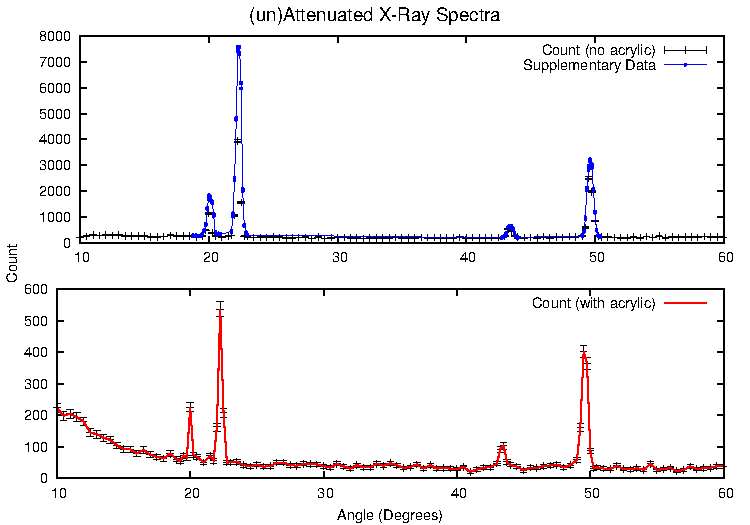
\includegraphics{XRaySpec-Angle.pdf}
\caption{The top plot includes higher angular resolution data (in blue) to illustrate more clearly the location of the peaks. Additionally, multiple sets of counts were collected for each high resolution angle to verify that the variance in measurements was at least Poissonian. The bottom plot shows the data obtained for measurements of every degree with the acrylic slide in place. Uncertainties in the angle measurements are not included here to keep the plots uncluttered.}
\label{fig:xrcg1}
\end{figure}

\item {\bf A graph of counts versus wavelength in nanometers with error bars for both x-ray spectra.}\newline

See Figure \ref{fig:xrcg2}.

\begin{figure}
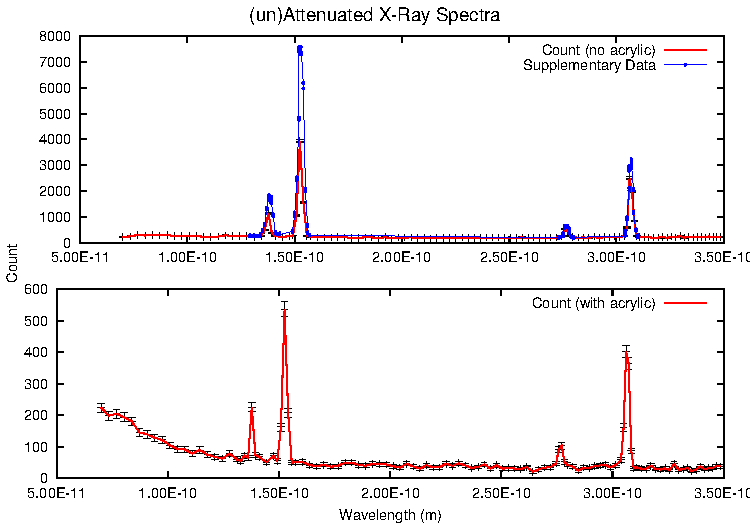
\includegraphics{XRaySpec-Wavelength.pdf}
\caption{This plot shows the wavelength (m) of the characteristic peaks of copper with and without the acrylic slide. Supplementary data is in blue.}
\label{fig:xrcg2}
\end{figure}

\item {\bf A graph of counts versus energy in keV with error bars for both x-ray spectra.}\newline

See Figure \ref{fig:xrcg3}.

\begin{figure}
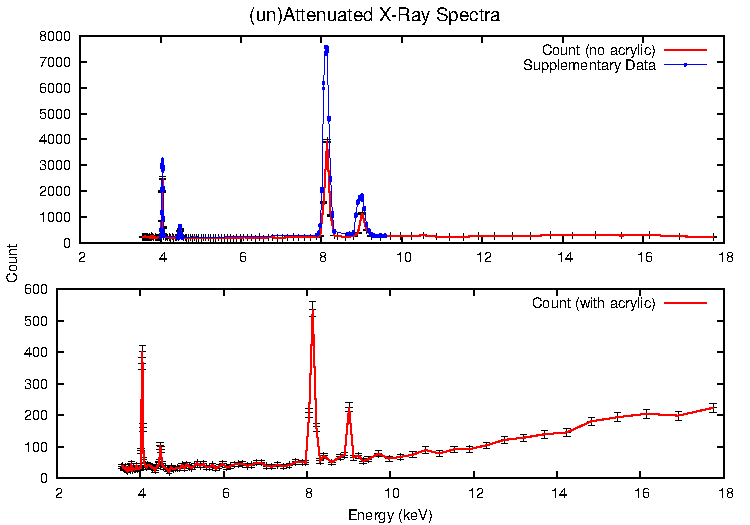
\includegraphics{XRaySpec-Energy.pdf}
\caption{This plot shows the energies (keV) of the characteristic peaks of copper with and without the acrylic slide. Supplementary data is in blue. The cut-off energy cannot be seen due to the physical constraints of the equipment. }
\label{fig:xrcg3}
\end{figure}

\item {\bf A value, with error, for the estimated cut-off wavelength, $\lambda_{min}$, of the of the x-ray tube.}\newline

Depending on the condition of the Bragg spectrometer that students use there may be varying degrees of success in obtaining a satisfactory data set for determining the cut-off energy. Ideally, students will obtain a spectrum such as that shown in Figure \ref{fig:xrcg4} from which they can discern the cut-off angle and thus the cut-off energy. It is likely that many won't however and so it is necessary to record appropriate magnitudes of uncertainty in extrapolations of the graph. 

Using the data from Figure \ref{fig:xrcg4} we estimate the cut-off angle to be 6$\pm$1$^{\circ}$. This corresponds to a wavelength of 42.1$\pm$6.99 picometers

\begin{figure}
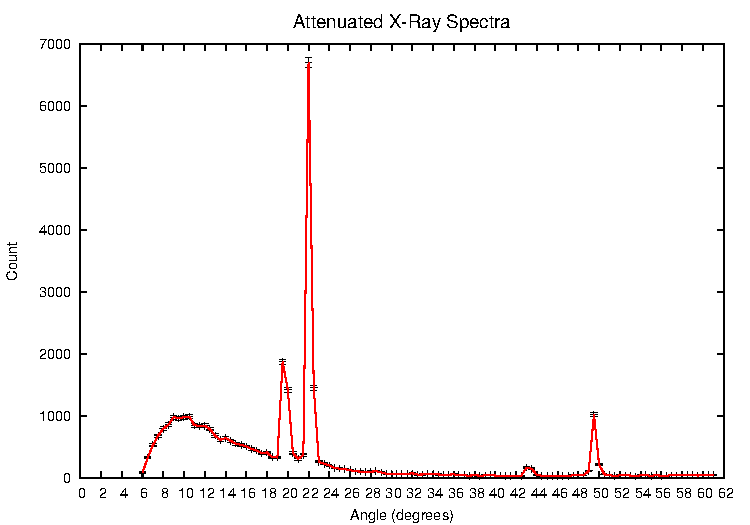
\includegraphics{HugoData-Angle.pdf}
\caption{Ideal spectrum for experimentally determining the cut-off energy of the Bragg x-ray spectrometer. Here the cut-off angle is easily extrapolated from the plot.}
\label{fig:xrcg4}
\end{figure}

\item {\bf A value, with error, for Planck's constant as derived from the cut-off wavelength.}\newline

The Planck constant can be calculated as follows,

\begin{equation}
h=\dfrac{eV}{c}\cdot 2d\cdot sin(\theta_{min})=4.208\times10^{-15}
\label{equ:twcg3}
\end{equation}

\noindent Where $eV$ is 30 keV corresponding to the spectrometer's energy setting and $\theta_{min}$ is the value extrapolated from the graph. The uncertainty is found from

\begin{equation}
u(h)=\dfrac{eV}{c}\cdot 2d\cdot cos(\theta_{min})\cdot u(\theta_{min})=6.988\times10^{-16}
\label{equ:twcg4}
\end{equation}

\item {\bf Values, with error, for the observed K-shell characteristic x-rays of copper.}\newline

The two values desired here are for K$_{\alpha}$ and K$_{\beta}$ (see Figure blah). K$_{\alpha}$ is actually a doublet but it is beyond the ability of this spectrometer to resolve it so we take the average value of the doublet to be E=8.038 keV. The energy of K$_{\beta}$ is taken to be E=8.905 keV. 

Reading from our data (see Tables \ref{tab:xrcg1}-\ref{tab:xrcg3} we see that the highest counts are obtained at energies of 8.139$\pm$ 0.174 keV and 9.010$\pm$0.216 keV. This gives us percent errors of 1.26\% for the K$_{\alpha}$ line and 1.18\% for the K$_{\beta}$ line. These values are well within experimental uncertainty. Accepted values for the characteristic energies of copper can be found in the Handbook of Chemistry and Physics, CRC Press, available online.


\end{enumerate}


\section{Discussion}
\begin{enumerate}[resume]

\item {\bf A comparison of the observed x-ray spectrum with the expected spectrum.}\newline

In our spectrum we see evidence of the expected braking radiation, smoothly spread across all energies and ending at the cut-off energy of the spectrometer. We also see the first and second order characteristic spikes of copper at the expected energies. We do not, however, see the K$_{\alpha}$ doublet. This is likely beyond the resolution of the spectrometer because of its relatively large beam width.

\item {\bf A comparison of the observed x-ray spectrum with the observed x-ray spectrum with the plastic inserted.}\newline

We again see the characteristic energy spikes of copper in their expected positions. Regarding the braking radiation, the right-skewed shape is more prominent when we attenuate the lower energy x-rays with the acrylic slide. This makes it somewhat easier to extrapolate the curve towards the cut-off energy (see Figure \ref{fig:xrcg4}).

\item {\bf A comparison of the observed cut-off and derived Planck's constant with the expected values.}\newline

Experimentally determined values for the cut-off energy (29.482$\pm$4.896 keV) and the Planck constant (4.208$\times$10$^{-15}\pm$6.988$\times$10$^{-16}$ eV s) agreed with literature values (30 keV and 4.136$\times$10$^{-15}$ eV s, respectively) to within uncertainty.

\item {\bf A comparison of the K-shell characteristic x-rays of copper with the accepted values.}\newline

Reading from our data (see Tables \ref{tab:xrcg1}-\ref{tab:xrcg3} we see that the highest counts are obtained at energies of 8.139$\pm$ 0.174 keV and 9.010$\pm$0.216 keV. This gives us percent errors of 1.26\% for the K$_{\alpha}$ line and 1.18\% for the K$_{\beta}$ line. These values are well within experimental uncertainty. Accepted values for the characteristic energies of copper can be found in the CRC Handbook, available online.

\item {\bf Discuss whether your results support or refute the hypothesis that x-rays are electromagnetic waves produced in the copper target of the x-ray tube by bremsstrahlung and K-shell interactions and diffracted by the LiF crystal.}\newline

All the predictions made under the assumption of the correctness of electromagnetic and spectroscopic theory as presented in this lab are supported by our results to within experimental uncertainties.

\item {\bf Using your results, explain why the third and fourth (if visible) peaks are more more likely to be n=2 versions of the first two peaks rather than separate characteristic x-rays.}\newline

Because the K$_{\beta}$ line is only $\sim$73 keV away from the ionization energy for copper we would expect that any higher energy lines would need to be very tightly packed and immediately following the K$_{\beta}$ line and at lower angles, i.e., higher energy. This is not what we see from the second set of lines in our spectra. These lines are at higher angles and lower energy. Given that the K$_{\alpha}$ line is predicted to be a transition from n=2 to n=1 we would expect no characteristic lines to be found at lower energies than K$_{\alpha}$. This leaves one possibility; the additional lines seen are the result of higher order diffraction.

\item {\bf The method of tilting a grating at an extreme angle to effectively get a very small spacing between lines is called the {\bf grazing incidence technique}. Figure 10 shows a tilted grating with distance AB between adjacent grooves. Calculate the angle $\theta$ required so that the effective grating spacing BC is 1/1000th the spacing of AB.}\newline

The effective spacing, d$_{eff}$, is given by,

\begin{equation}
d_{eff}=dsin(\theta)
\label{equ:twcg5}
\end{equation}

\noindent We want d$_{eff}$ to be d/1000.

\begin{equation}
\dfrac{d}{1000}=dsin(\theta)
\label{equ:twcg6}
\end{equation}

\begin{equation}
\theta=sin^{-1}\left(\dfrac{1}{1000}\right)=0.057^{\circ}
\label{equ:twcg7}
\end{equation}

So the minimum angle necessary to achieve a line spacing that is 1/1000$^{th}$ of the original, AB, is 0.057$^{\circ}$.

\end{enumerate}
\newpage

\begin{table}[ht]
\center
\begin{tabular}{cccccccccc}
\multicolumn{1}{c}{2$\theta$} & \multicolumn{1}{c}{u(2$\theta$)} & \multicolumn{1}{c}{$\theta$} & \multicolumn{1}{c}{u($\theta$)} & \multicolumn{1}{c}{Count} & \multicolumn{1}{c}{u(Count)} & \multicolumn{1}{c}{$\lambda$ (m)} & \multicolumn{1}{c}{u($\lambda$) (m)} & \multicolumn{1}{c}{Energy (keV)} & \multicolumn{1}{c}{u(Energy) (keV)} \\
20          & 1.0   & 10         & 0.5           & 217     & 14.7       & 6.99E-11    & 3.46E-12       & 17.7469   & 0.8783       \\
21          & 1.0   & 10.5       & 0.5           & 247     & 15.7       & 7.34E-11    & 3.45E-12       & 16.9106   & 0.7962       \\
22          & 1.0   & 11         & 0.5           & 300     & 17.3       & 7.68E-11    & 3.45E-12       & 16.1508   & 0.7251       \\
23          & 1.0   & 11.5       & 0.5           & 279     & 16.7       & 8.03E-11    & 3.44E-12       & 15.4574   & 0.6630       \\
24          & 1.0   & 12         & 0.5           & 300     & 17.3       & 8.37E-11    & 3.44E-12       & 14.8223   & 0.6085       \\
25          & 1.0   & 12.5       & 0.5           & 288     & 17.0       & 8.71E-11    & 3.43E-12       & 14.2382   & 0.5605       \\
26          & 1.0   & 13         & 0.5           & 303     & 17.4       & 9.06E-11    & 3.42E-12       & 13.6995   & 0.5178       \\
27          & 1.0   & 13.5       & 0.5           & 256     & 16.0       & 9.40E-11    & 3.42E-12       & 13.2010   & 0.4798       \\
28          & 1.0   & 14         & 0.5           & 253     & 15.9       & 9.74E-11    & 3.41E-12       & 12.7385   & 0.4459       \\
29          & 1.0   & 14.5       & 0.5           & 255     & 16.0       & 1.01E-10    & 3.40E-12       & 12.3082   & 0.4153       \\
30          & 1.0   & 15         & 0.5           & 257     & 16.0       & 1.04E-10    & 3.39E-12       & 11.9069   & 0.3878       \\
31          & 1.0   & 15.5       & 0.5           & 232     & 15.2       & 1.08E-10    & 3.39E-12       & 11.5317   & 0.3629       \\
32          & 1.0   & 16         & 0.5           & 227     & 15.1       & 1.11E-10    & 3.38E-12       & 11.1803   & 0.3403       \\
33          & 1.0   & 16.5       & 0.5           & 240     & 15.5       & 1.14E-10    & 3.37E-12       & 10.8505   & 0.3197       \\
34          & 1.0   & 17         & 0.5           & 286     & 16.9       & 1.18E-10    & 3.36E-12       & 10.5404   & 0.3009       \\
35          & 1.0   & 17.5       & 0.5           & 261     & 16.2       & 1.21E-10    & 3.35E-12       & 10.2483   & 0.2836       \\
36          & 1.0   & 18         & 0.5           & 256     & 16.0       & 1.24E-10    & 3.34E-12       & 9.9727    & 0.2678       \\
37          & 1.0   & 18.5       & 0.5           & 263     & 16.2       & 1.28E-10    & 3.33E-12       & 9.7122    & 0.2533       \\
38          & 1.0   & 19         & 0.5           & 225     & 15.0       & 1.31E-10    & 3.32E-12       & 9.4657    & 0.2399       \\
39          & 1.0   & 19.5       & 0.5           & 269     & 16.4       & 1.34E-10    & 3.31E-12       & 9.2320    & 0.2275       \\
39.5        & 1.0   & 19.75      & 0.5           & 491     & 22.2       & 1.36E-10    & 3.31E-12       & 9.1198    & 0.2217       \\
40          & 1.0   & 20         & 0.5           & 1143    & 33.8       & 1.38E-10    & 3.30E-12       & 9.0103    & 0.2160       \\
40.5        & 1.0   & 20.25      & 0.5           & 373     & 19.3       & 1.39E-10    & 3.30E-12       & 8.9037    & 0.2106       \\
41          & 1.0   & 20.5       & 0.5           & 250     & 15.8       & 1.41E-10    & 3.29E-12       & 8.7997    & 0.2054       \\
42          & 1.0   & 21         & 0.5           & 231     & 15.2       & 1.44E-10    & 3.28E-12       & 8.5993    & 0.1955       \\
43          & 1.0   & 21.5       & 0.5           & 249     & 15.8       & 1.48E-10    & 3.27E-12       & 8.4085    & 0.1863       \\
43.5        & 1.0   & 21.75      & 0.5           & 280     & 16.7       & 1.49E-10    & 3.26E-12       & 8.3164    & 0.1819       \\
44          & 1.0   & 22         & 0.5           & 1056    & 32.5       & 1.51E-10    & 3.26E-12       & 8.2265    & 0.1777       \\
44.5        & 1.0   & 22.25      & 0.5           & 3936    & 62.7       & 1.52E-10    & 3.25E-12       & 8.1387    & 0.1736       \\
45          & 1.0   & 22.5       & 0.5           & 1552    & 39.4       & 1.54E-10    & 3.25E-12       & 8.0529    & 0.1697       \\
45.5        & 1.0   & 22.75      & 0.5           & 253     & 15.9       & 1.56E-10    & 3.24E-12       & 7.9691    & 0.1658       \\
46          & 1.0   & 23         & 0.5           & 235     & 15.3       & 1.57E-10    & 3.23E-12       & 7.8871    & 0.1621       \\
47          & 1.0   & 23.5       & 0.5           & 200     & 14.1       & 1.61E-10    & 3.22E-12       & 7.7285    & 0.1551       \\
48          & 1.0   & 24         & 0.5           & 209     & 14.5       & 1.64E-10    & 3.21E-12       & 7.5767    & 0.1485       \\
49          & 1.0   & 24.5       & 0.5           & 207     & 14.4       & 1.67E-10    & 3.20E-12       & 7.4313    & 0.1423       \\
50          & 1.0   & 25         & 0.5           & 228     & 15.1       & 1.70E-10    & 3.18E-12       & 7.2920    & 0.1365       \\
51          & 1.0   & 25.5       & 0.5           & 210     & 14.5       & 1.73E-10    & 3.17E-12       & 7.1583    & 0.1310       \\
52          & 1.0   & 26         & 0.5           & 189     & 13.7       & 1.76E-10    & 3.16E-12       & 7.0299    & 0.1258       \\
53          & 1.0   & 26.5       & 0.5           & 191     & 13.8       & 1.80E-10    & 3.14E-12       & 6.9066    & 0.1209       \\
54          & 1.0   & 27         & 0.5           & 204     & 14.3       & 1.83E-10    & 3.13E-12       & 6.7881    & 0.1163       \\
55          & 1.0   & 27.5       & 0.5           & 207     & 14.4       & 1.86E-10    & 3.12E-12       & 6.6740    & 0.1119       \\
56          & 1.0   & 28         & 0.5           & 170     & 13.0       & 1.89E-10    & 3.10E-12       & 6.5642    & 0.1077       \\
57          & 1.0   & 28.5       & 0.5           & 214     & 14.6       & 1.92E-10    & 3.09E-12       & 6.4585    & 0.1038       \\
58          & 1.0   & 29         & 0.5           & 170     & 13.0       & 1.95E-10    & 3.07E-12       & 6.3566    & 0.1001       \\
59          & 1.0   & 29.5       & 0.5           & 193     & 13.9       & 1.98E-10    & 3.06E-12       & 6.2583    & 0.0965       \\
60          & 1.0   & 30         & 0.5           & 199     & 14.1       & 2.01E-10    & 3.04E-12       & 6.1634    & 0.0932       \\
\end{tabular}
\caption{Data for unattenuated x-rays.}
\label{tab:xrcg1}
\end{table}



\begin{table}[ht]
\center
\begin{tabular}{cccccccccc}
\multicolumn{1}{c}{2$\theta$} & \multicolumn{1}{c}{u(2$\theta$)} & \multicolumn{1}{c}{$\theta$} & \multicolumn{1}{c}{u($\theta$)} & \multicolumn{1}{c}{Count} & \multicolumn{1}{c}{u(Count)} & \multicolumn{1}{c}{$\lambda$ (m)} & \multicolumn{1}{c}{u($\lambda$) (m)} & \multicolumn{1}{c}{Energy (keV)} & \multicolumn{1}{c}{u(Energy) (keV)} \\
61          & 1.0   & 30.5       & 0.5           & 204     & 14.3       & 2.04E-10    & 3.03E-12       & 6.0719    & 0.0900       \\
62          & 1.0   & 31         & 0.5           & 182     & 13.5       & 2.07E-10    & 3.01E-12       & 5.9835    & 0.0869       \\
63          & 1.0   & 31.5       & 0.5           & 186     & 13.6       & 2.10E-10    & 3.00E-12       & 5.8980    & 0.0840       \\
64          & 1.0   & 32         & 0.5           & 170     & 13.0       & 2.13E-10    & 2.98E-12       & 5.8155    & 0.0812       \\
65          & 1.0   & 32.5       & 0.5           & 184     & 13.6       & 2.16E-10    & 2.96E-12       & 5.7356    & 0.0786       \\
66          & 1.0   & 33         & 0.5           & 178     & 13.3       & 2.19E-10    & 2.95E-12       & 5.6583    & 0.0760       \\
67          & 1.0   & 33.5       & 0.5           & 173     & 13.2       & 2.22E-10    & 2.93E-12       & 5.5835    & 0.0736       \\
68          & 1.0   & 34         & 0.5           & 183     & 13.5       & 2.25E-10    & 2.91E-12       & 5.5110    & 0.0713       \\
69          & 1.0   & 34.5       & 0.5           & 205     & 14.3       & 2.28E-10    & 2.90E-12       & 5.4408    & 0.0691       \\
70          & 1.0   & 35         & 0.5           & 178     & 13.3       & 2.31E-10    & 2.88E-12       & 5.3728    & 0.0670       \\
71          & 1.0   & 35.5       & 0.5           & 190     & 13.8       & 2.34E-10    & 2.86E-12       & 5.3069    & 0.0649       \\
72          & 1.0   & 36         & 0.5           & 180     & 13.4       & 2.37E-10    & 2.84E-12       & 5.2429    & 0.0630       \\
73          & 1.0   & 36.5       & 0.5           & 198     & 14.1       & 2.39E-10    & 2.82E-12       & 5.1809    & 0.0611       \\
74          & 1.0   & 37         & 0.5           & 195     & 14.0       & 2.42E-10    & 2.81E-12       & 5.1207    & 0.0593       \\
75          & 1.0   & 37.5       & 0.5           & 194     & 13.9       & 2.45E-10    & 2.79E-12       & 5.0623    & 0.0576       \\
76          & 1.0   & 38         & 0.5           & 181     & 13.5       & 2.48E-10    & 2.77E-12       & 5.0055    & 0.0559       \\
77          & 1.0   & 38.5       & 0.5           & 179     & 13.4       & 2.51E-10    & 2.75E-12       & 4.9504    & 0.0543       \\
78          & 1.0   & 39         & 0.5           & 175     & 13.2       & 2.53E-10    & 2.73E-12       & 4.8969    & 0.0528       \\
79          & 1.0   & 39.5       & 0.5           & 212     & 14.6       & 2.56E-10    & 2.71E-12       & 4.8449    & 0.0513       \\
80          & 1.0   & 40         & 0.5           & 175     & 13.2       & 2.59E-10    & 2.69E-12       & 4.7943    & 0.0499       \\
81          & 1.0   & 40.5       & 0.5           & 193     & 13.9       & 2.61E-10    & 2.67E-12       & 4.7451    & 0.0485       \\
82          & 1.0   & 41         & 0.5           & 173     & 13.2       & 2.64E-10    & 2.65E-12       & 4.6973    & 0.0472       \\
83          & 1.0   & 41.5       & 0.5           & 187     & 13.7       & 2.67E-10    & 2.63E-12       & 4.6508    & 0.0459       \\
84          & 1.0   & 42         & 0.5           & 193     & 13.9       & 2.69E-10    & 2.61E-12       & 4.6056    & 0.0446       \\
85          & 1.0   & 42.5       & 0.5           & 195     & 14.0       & 2.72E-10    & 2.59E-12       & 4.5615    & 0.0434       \\
86          & 1.0   & 43         & 0.5           & 258     & 16.1       & 2.75E-10    & 2.57E-12       & 4.5187    & 0.0423       \\
86.5        & 1.0   & 43.25      & 0.5           & 518     & 22.8       & 2.76E-10    & 2.56E-12       & 4.4977    & 0.0417       \\
87          & 1.0   & 43.5       & 0.5           & 449     & 21.2       & 2.77E-10    & 2.55E-12       & 4.4769    & 0.0412       \\
87.5        & 1.0   & 43.75      & 0.5           & 273     & 16.5       & 2.78E-10    & 2.54E-12       & 4.4565    & 0.0406       \\
88          & 1.0   & 44         & 0.5           & 221     & 14.9       & 2.80E-10    & 2.53E-12       & 4.4363    & 0.0401       \\
89          & 1.0   & 44.5       & 0.5           & 194     & 13.9       & 2.82E-10    & 2.51E-12       & 4.3967    & 0.0390       \\
90          & 1.0   & 45         & 0.5           & 204     & 14.3       & 2.85E-10    & 2.48E-12       & 4.3582    & 0.0380       \\
91          & 1.0   & 45.5       & 0.5           & 185     & 13.6       & 2.87E-10    & 2.46E-12       & 4.3207    & 0.0371       \\
92          & 1.0   & 46         & 0.5           & 235     & 15.3       & 2.90E-10    & 2.44E-12       & 4.2841    & 0.0361       \\
93          & 1.0   & 46.5       & 0.5           & 176     & 13.3       & 2.92E-10    & 2.42E-12       & 4.2485    & 0.0352       \\
94          & 1.0   & 47         & 0.5           & 215     & 14.7       & 2.94E-10    & 2.40E-12       & 4.2137    & 0.0343       \\
95          & 1.0   & 47.5       & 0.5           & 211     & 14.5       & 2.97E-10    & 2.37E-12       & 4.1799    & 0.0334       \\
96          & 1.0   & 48         & 0.5           & 233     & 15.3       & 2.99E-10    & 2.35E-12       & 4.1469    & 0.0326       \\
97          & 1.0   & 48.5       & 0.5           & 222     & 14.9       & 3.02E-10    & 2.33E-12       & 4.1147    & 0.0318       \\
98          & 1.0   & 49         & 0.5           & 255     & 16.0       & 3.04E-10    & 2.30E-12       & 4.0833    & 0.0310       \\
98.5        & 1.0   & 49.25      & 0.5           & 592     & 24.3       & 3.05E-10    & 2.29E-12       & 4.0679    & 0.0306       \\
99          & 1.0   & 49.5       & 0.5           & 2502    & 50.0       & 3.06E-10    & 2.28E-12       & 4.0527    & 0.0302       \\
99.5        & 1.0   & 49.75      & 0.5           & 1975    & 44.4       & 3.07E-10    & 2.27E-12       & 4.0377    & 0.0298       \\
100         & 1.0   & 50         & 0.5           & 837     & 28.9       & 3.08E-10    & 2.26E-12       & 4.0229    & 0.0295       \\
100.5       & 1.0   & 50.25      & 0.5           & 252     & 15.9       & 3.10E-10    & 2.25E-12       & 4.0083    & 0.0291       \\
\end{tabular}
\caption{Data for unattenuated x-rays.}
\label{tab:xrcg2}
\end{table}



\begin{table}[ht]
\center
\begin{tabular}{cccccccccc}
\multicolumn{1}{c}{2$\theta$} & \multicolumn{1}{c}{u(2$\theta$)} & \multicolumn{1}{c}{$\theta$} & \multicolumn{1}{c}{u($\theta$)} & \multicolumn{1}{c}{Count} & \multicolumn{1}{c}{u(Count)} & \multicolumn{1}{c}{$\lambda$ (m)} & \multicolumn{1}{c}{u($\lambda$) (m)} & \multicolumn{1}{c}{Energy (keV)} & \multicolumn{1}{c}{u(Energy) (keV)} \\
101         & 1.0   & 50.5       & 0.5           & 219     & 14.8       & 3.11E-10    & 2.23E-12       & 3.9938    & 0.0287       \\
102         & 1.0   & 51         & 0.5           & 224     & 15.0       & 3.13E-10    & 2.21E-12       & 3.9654    & 0.0280       \\
103         & 1.0   & 51.5       & 0.5           & 205     & 14.3       & 3.15E-10    & 2.19E-12       & 3.9378    & 0.0273       \\
104         & 1.0   & 52         & 0.5           & 196     & 14.0       & 3.17E-10    & 2.16E-12       & 3.9108    & 0.0267       \\
105         & 1.0   & 52.5       & 0.5           & 196     & 14.0       & 3.19E-10    & 2.14E-12       & 3.8844    & 0.0260       \\
106         & 1.0   & 53         & 0.5           & 216     & 14.7       & 3.22E-10    & 2.11E-12       & 3.8587    & 0.0254       \\
107         & 1.0   & 53.5       & 0.5           & 194     & 13.9       & 3.24E-10    & 2.09E-12       & 3.8337    & 0.0248       \\
108         & 1.0   & 54         & 0.5           & 238     & 15.4       & 3.26E-10    & 2.07E-12       & 3.8092    & 0.0242       \\
109         & 1.0   & 54.5       & 0.5           & 204     & 14.3       & 3.28E-10    & 2.04E-12       & 3.7854    & 0.0236       \\
110         & 1.0   & 55         & 0.5           & 255     & 16.0       & 3.30E-10    & 2.02E-12       & 3.7621    & 0.0230       \\
111         & 1.0   & 55.5       & 0.5           & 193     & 13.9       & 3.32E-10    & 1.99E-12       & 3.7394    & 0.0224       \\
112         & 1.0   & 56         & 0.5           & 231     & 15.2       & 3.34E-10    & 1.96E-12       & 3.7172    & 0.0219       \\
113         & 1.0   & 56.5       & 0.5           & 212     & 14.6       & 3.36E-10    & 1.94E-12       & 3.6956    & 0.0213       \\
114         & 1.0   & 57         & 0.5           & 214     & 14.6       & 3.38E-10    & 1.91E-12       & 3.6745    & 0.0208       \\
115         & 1.0   & 57.5       & 0.5           & 213     & 14.6       & 3.40E-10    & 1.89E-12       & 3.6540    & 0.0203       \\
116         & 1.0   & 58         & 0.5           & 208     & 14.4       & 3.41E-10    & 1.86E-12       & 3.6339    & 0.0198       \\
117         & 1.0   & 58.5       & 0.5           & 243     & 15.6       & 3.43E-10    & 1.84E-12       & 3.6143    & 0.0193       \\
118         & 1.0   & 59         & 0.5           & 221     & 14.9       & 3.45E-10    & 1.81E-12       & 3.5952    & 0.0189       \\
119         & 1.0   & 59.5       & 0.5           & 225     & 15.0       & 3.47E-10    & 1.78E-12       & 3.5766    & 0.0184       \\
120         & 1.0   & 60         & 0.5           & 219     & 14.8       & 3.49E-10    & 1.76E-12       & 3.5585    & 0.0179      
\end{tabular}
\caption{Data for unattenuated x-rays.}
\label{tab:xrcg3}
\end{table}



\begin{table}[ht]
\center
\begin{tabular}{cccccccccc}
2$\theta$ & u(2$\theta$) & $\theta$ & u($\theta$) & Count & u(Count) & $\lambda$ (m) & u($\lambda$) (m) & Energy (keV) & u(Energy) (keV) \\
20        & 1.0 & 10       & 0.5         & 224   & 15.0     & 6.99E-11      & 3.46E-12         & 17.7469      & 0.8783 \\
21        & 1.0 & 10.5     & 0.5         & 199   & 14.1     & 7.34E-11      & 3.45E-12         & 16.9106      & 0.7962 \\
22        & 1.0 & 11       & 0.5         & 205   & 14.3     & 7.68E-11      & 3.45E-12         & 16.1508      & 0.7251 \\
23        & 1.0 & 11.5     & 0.5         & 194   & 13.9     & 8.03E-11      & 3.44E-12         & 15.4574      & 0.6630 \\
24        & 1.0 & 12       & 0.5         & 181   & 13.5     & 8.37E-11      & 3.44E-12         & 14.8223      & 0.6085 \\
25        & 1.0 & 12.5     & 0.5         & 146   & 12.1     & 8.71E-11      & 3.43E-12         & 14.2382      & 0.5605 \\
26        & 1.0 & 13       & 0.5         & 140   & 11.8     & 9.06E-11      & 3.42E-12         & 13.6995      & 0.5178 \\
27        & 1.0 & 13.5     & 0.5         & 129   & 11.4     & 9.40E-11      & 3.42E-12         & 13.2010      & 0.4798 \\
28        & 1.0 & 14       & 0.5         & 122   & 11.0     & 9.74E-11      & 3.41E-12         & 12.7385      & 0.4459 \\
29        & 1.0 & 14.5     & 0.5         & 105   & 10.2     & 1.01E-10      & 3.40E-12         & 12.3082      & 0.4153 \\
30        & 1.0 & 15       & 0.5         & 93    & 9.6      & 1.04E-10      & 3.39E-12         & 11.9069      & 0.3878 \\
31        & 1.0 & 15.5     & 0.5         & 92    & 9.6      & 1.08E-10      & 3.39E-12         & 11.5317      & 0.3629 \\
32        & 1.0 & 16       & 0.5         & 79    & 8.9      & 1.11E-10      & 3.38E-12         & 11.1803      & 0.3403 \\
33        & 1.0 & 16.5     & 0.5         & 90    & 9.5      & 1.14E-10      & 3.37E-12         & 10.8505      & 0.3197 \\
34        & 1.0 & 17       & 0.5         & 75    & 8.7      & 1.18E-10      & 3.36E-12         & 10.5404      & 0.3009 \\
35        & 1.0 & 17.5     & 0.5         & 68    & 8.2      & 1.21E-10      & 3.35E-12         & 10.2483      & 0.2836 \\
36        & 1.0 & 18       & 0.5         & 63    & 7.9      & 1.24E-10      & 3.34E-12         & 9.9727       & 0.2678 \\
37        & 1.0 & 18.5     & 0.5         & 78    & 8.8      & 1.28E-10      & 3.33E-12         & 9.7122       & 0.2533 \\
38        & 1.0 & 19       & 0.5         & 60    & 7.7      & 1.31E-10      & 3.32E-12         & 9.4657       & 0.2399 \\
38.5        & 1.0 & 19.25    & 0.5         & 55    & 7.4      & 1.33E-10      & 3.32E-12         & 9.3473       & 0.2336 \\
39        & 1.0 & 19.5     & 0.5         & 72    & 8.5      & 1.34E-10      & 3.31E-12         & 9.2320       & 0.2275 \\
39.5        & 1.0 & 19.75    & 0.5         & 66    & 8.1      & 1.36E-10      & 3.31E-12         & 9.1198       & 0.2217 \\
40        & 1.0 & 20       & 0.5         & 226   & 15.0     & 1.38E-10      & 3.30E-12         & 9.0103       & 0.2160 \\
40.5        & 1.0 & 20.25    & 0.5         & 74    & 8.6      & 1.39E-10      & 3.30E-12         & 8.9037       & 0.2106 \\
41        & 1.0 & 20.5     & 0.5         & 68    & 8.2      & 1.41E-10      & 3.29E-12         & 8.7997       & 0.2054 \\
42        & 1.0 & 21       & 0.5         & 51    & 7.1      & 1.44E-10      & 3.28E-12         & 8.5993       & 0.1955 \\
43        & 1.0 & 21.5     & 0.5         & 71    & 8.4      & 1.48E-10      & 3.27E-12         & 8.4085       & 0.1863 \\
43.5        & 1.0 & 21.75    & 0.5         & 56    & 7.5      & 1.49E-10      & 3.26E-12         & 8.3164       & 0.1819 \\
44        & 1.0 & 22       & 0.5         & 163   & 12.8     & 1.51E-10      & 3.26E-12         & 8.2265       & 0.1777 \\
44.5        & 1.0 & 22.25    & 0.5         & 537   & 23.2     & 1.52E-10      & 3.25E-12         & 8.1387       & 0.1736 \\
45        & 1.0 & 22.5     & 0.5         & 208   & 14.4     & 1.54E-10      & 3.25E-12         & 8.0529       & 0.1697 \\
45.5        & 1.0 & 22.75    & 0.5         & 50    & 7.1      & 1.56E-10      & 3.24E-12         & 7.9691       & 0.1658 \\
46        & 1.0 & 23       & 0.5         & 51    & 7.1      & 1.57E-10      & 3.23E-12         & 7.8871       & 0.1621 \\
47        & 1.0 & 23.5     & 0.5         & 52    & 7.2      & 1.61E-10      & 3.22E-12         & 7.7285       & 0.1551 \\
48        & 1.0 & 24       & 0.5         & 42    & 6.5      & 1.64E-10      & 3.21E-12         & 7.5767       & 0.1485 \\
49        & 1.0 & 24.5     & 0.5         & 38    & 6.2      & 1.67E-10      & 3.20E-12         & 7.4313       & 0.1423 \\
50        & 1.0 & 25       & 0.5         & 43    & 6.6      & 1.70E-10      & 3.18E-12         & 7.2920       & 0.1365 \\
51        & 1.0 & 25.5     & 0.5         & 37    & 6.1      & 1.73E-10      & 3.17E-12         & 7.1583       & 0.1310 \\
52        & 1.0 & 26       & 0.5         & 39    & 6.2      & 1.76E-10      & 3.16E-12         & 7.0299       & 0.1258 \\
53        & 1.0 & 26.5     & 0.5         & 50    & 7.1      & 1.80E-10      & 3.14E-12         & 6.9066       & 0.1209 \\
54        & 1.0 & 27       & 0.5         & 50    & 7.1      & 1.83E-10      & 3.13E-12         & 6.7881       & 0.1163 \\
55        & 1.0 & 27.5     & 0.5         & 42    & 6.5      & 1.86E-10      & 3.12E-12         & 6.6740       & 0.1119 \\
56        & 1.0 & 28       & 0.5         & 40    & 6.3      & 1.89E-10      & 3.10E-12         & 6.5642       & 0.1077 \\
57        & 1.0 & 28.5     & 0.5         & 46    & 6.8      & 1.92E-10      & 3.09E-12         & 6.4585       & 0.1038 \\
58        & 1.0 & 29       & 0.5         & 45    & 6.7      & 1.95E-10      & 3.07E-12         & 6.3566       & 0.1001 \\
59        & 1.0 & 29.5     & 0.5         & 44    & 6.6      & 1.98E-10      & 3.06E-12         & 6.2583       & 0.0965 \\
60        & 1.0 & 30       & 0.5         & 39    & 6.2      & 2.01E-10      & 3.04E-12         & 6.1634       & 0.0932 \\
\end{tabular}
\caption{Data for x-rays attenuated by an acrylic slide.}
\label{tab:xrcg4}
\end{table}



\begin{table}[ht]
\center
\begin{tabular}{cccccccccc}
2$\theta$ & u(2$\theta$) & $\theta$ & u($\theta$) & Count & u(Count) & $\lambda$ (m) & u($\lambda$) (m) & Energy (keV) & u(Energy) (keV) \\
61        & 1.0 & 30.5     & 0.5         & 34    & 5.8      & 2.04E-10      & 3.03E-12         & 6.0719       & 0.0900 \\
62        & 1.0 & 31       & 0.5         & 46    & 6.8      & 2.07E-10      & 3.01E-12         & 5.9835       & 0.0869 \\
63        & 1.0 & 31.5     & 0.5         & 38    & 6.2      & 2.10E-10      & 3.00E-12         & 5.8980       & 0.0840 \\
64        & 1.0 & 32       & 0.5         & 31    & 5.6      & 2.13E-10      & 2.98E-12         & 5.8155       & 0.0812 \\
65        & 1.0 & 32.5     & 0.5         & 42    & 6.5      & 2.16E-10      & 2.96E-12         & 5.7356       & 0.0786 \\
66        & 1.0 & 33       & 0.5         & 35    & 5.9      & 2.19E-10      & 2.95E-12         & 5.6583       & 0.0760 \\
67        & 1.0 & 33.5     & 0.5         & 35    & 5.9      & 2.22E-10      & 2.93E-12         & 5.5835       & 0.0736 \\
68        & 1.0 & 34       & 0.5         & 46    & 6.8      & 2.25E-10      & 2.91E-12         & 5.5110       & 0.0713 \\
69        & 1.0 & 34.5     & 0.5         & 40    & 6.3      & 2.28E-10      & 2.90E-12         & 5.4408       & 0.0691 \\
70        & 1.0 & 35       & 0.5         & 48    & 6.9      & 2.31E-10      & 2.88E-12         & 5.3728       & 0.0670 \\
71        & 1.0 & 35.5     & 0.5         & 41    & 6.4      & 2.34E-10      & 2.86E-12         & 5.3069       & 0.0649 \\
72        & 1.0 & 36       & 0.5         & 33    & 5.7      & 2.37E-10      & 2.84E-12         & 5.2429       & 0.0630 \\
73        & 1.0 & 36.5     & 0.5         & 36    & 6.0      & 2.39E-10      & 2.82E-12         & 5.1809       & 0.0611 \\
74        & 1.0 & 37       & 0.5         & 44    & 6.6      & 2.42E-10      & 2.81E-12         & 5.1207       & 0.0593 \\
75        & 1.0 & 37.5     & 0.5         & 31    & 5.6      & 2.45E-10      & 2.79E-12         & 5.0623       & 0.0576 \\
76        & 1.0 & 38       & 0.5         & 42    & 6.5      & 2.48E-10      & 2.77E-12         & 5.0055       & 0.0559 \\
77        & 1.0 & 38.5     & 0.5         & 31    & 5.6      & 2.51E-10      & 2.75E-12         & 4.9504       & 0.0543 \\
78        & 1.0 & 39       & 0.5         & 32    & 5.7      & 2.53E-10      & 2.73E-12         & 4.8969       & 0.0528 \\
79        & 1.0 & 39.5     & 0.5         & 31    & 5.6      & 2.56E-10      & 2.71E-12         & 4.8449       & 0.0513 \\
80        & 1.0 & 40       & 0.5         & 29    & 5.4      & 2.59E-10      & 2.69E-12         & 4.7943       & 0.0499 \\
81        & 1.0 & 40.5     & 0.5         & 36    & 6.0      & 2.61E-10      & 2.67E-12         & 4.7451       & 0.0485 \\
82        & 1.0 & 41       & 0.5         & 21    & 4.6      & 2.64E-10      & 2.65E-12         & 4.6973       & 0.0472 \\
83        & 1.0 & 41.5     & 0.5         & 28    & 5.3      & 2.67E-10      & 2.63E-12         & 4.6508       & 0.0459 \\
84        & 1.0 & 42       & 0.5         & 34    & 5.8      & 2.69E-10      & 2.61E-12         & 4.6056       & 0.0446 \\
85        & 1.0 & 42.5     & 0.5         & 35    & 5.9      & 2.72E-10      & 2.59E-12         & 4.5615       & 0.0434 \\
86        & 1.0 & 43       & 0.5         & 47    & 6.9      & 2.75E-10      & 2.57E-12         & 4.5187       & 0.0423 \\
86.5        & 1.0 & 43.25    & 0.5         & 93    & 9.6      & 2.76E-10      & 2.56E-12         & 4.4977       & 0.0417 \\
87        & 1.0 & 43.5     & 0.5         & 103   & 10.1     & 2.77E-10      & 2.55E-12         & 4.4769       & 0.0412 \\
87.5        & 1.0 & 43.75    & 0.5         & 52    & 7.2      & 2.78E-10      & 2.54E-12         & 4.4565       & 0.0406 \\
88        & 1.0 & 44       & 0.5         & 43    & 6.6      & 2.80E-10      & 2.53E-12         & 4.4363       & 0.0401 \\
89        & 1.0 & 44.5     & 0.5         & 37    & 6.1      & 2.82E-10      & 2.51E-12         & 4.3967       & 0.0390 \\
90        & 1.0 & 45       & 0.5         & 25    & 5.0      & 2.85E-10      & 2.48E-12         & 4.3582       & 0.0380 \\
91        & 1.0 & 45.5     & 0.5         & 34    & 5.8      & 2.87E-10      & 2.46E-12         & 4.3207       & 0.0371 \\
92        & 1.0 & 46       & 0.5         & 33    & 5.7      & 2.90E-10      & 2.44E-12         & 4.2841       & 0.0361 \\
93        & 1.0 & 46.5     & 0.5         & 39    & 6.2      & 2.92E-10      & 2.42E-12         & 4.2485       & 0.0352 \\
94        & 1.0 & 47       & 0.5         & 41    & 6.4      & 2.94E-10      & 2.40E-12         & 4.2137       & 0.0343 \\
95        & 1.0 & 47.5     & 0.5         & 43    & 6.6      & 2.97E-10      & 2.37E-12         & 4.1799       & 0.0334 \\
96        & 1.0 & 48       & 0.5         & 35    & 5.9      & 2.99E-10      & 2.35E-12         & 4.1469       & 0.0326 \\
97        & 1.0 & 48.5     & 0.5         & 42    & 6.5      & 3.02E-10      & 2.33E-12         & 4.1147       & 0.0318 \\
98        & 1.0 & 49       & 0.5         & 59    & 7.7      & 3.04E-10      & 2.30E-12         & 4.0833       & 0.0310 \\
98.5        & 1.0 & 49.25    & 0.5         & 162   & 12.7     & 3.05E-10      & 2.29E-12         & 4.0679       & 0.0306 \\
99        & 1.0 & 49.5     & 0.5         & 403   & 20.1     & 3.06E-10      & 2.28E-12         & 4.0527       & 0.0302 \\
99.5       & 1.0 & 49.75    & 0.5         & 365   & 19.1     & 3.07E-10      & 2.27E-12         & 4.0377       & 0.0298 \\
\end{tabular}
\caption{Data for x-rays attenuated by an acrylic slide.}
\label{tab:xrcg5}
\end{table}



\begin{table}[ht]
\center
\begin{tabular}{cccccccccc}
2$\theta$ & u(2$\theta$) & $\theta$ & u($\theta$) & Count & u(Count) & $\lambda$ (m) & u($\lambda$) (m) & Energy (keV) & u(Energy) (keV) \\
100       & 1.0 & 50       & 0.5         & 87    & 9.3      & 3.08E-10      & 2.26E-12         & 4.0229       & 0.0295 \\
100.5       & 1.0 & 50.25    & 0.5         & 31    & 5.6      & 3.10E-10      & 2.25E-12         & 4.0083       & 0.0291 \\
101       & 1.0 & 50.5     & 0.5         & 35    & 5.9      & 3.11E-10      & 2.23E-12         & 3.9938       & 0.0287 \\
102       & 1.0 & 51       & 0.5         & 31    & 5.6      & 3.13E-10      & 2.21E-12         & 3.9654       & 0.0280 \\
103       & 1.0 & 51.5     & 0.5         & 30    & 5.5      & 3.15E-10      & 2.19E-12         & 3.9378       & 0.0273 \\
104       & 1.0 & 52       & 0.5         & 40    & 6.3      & 3.17E-10      & 2.16E-12         & 3.9108       & 0.0267 \\
105       & 1.0 & 52.5     & 0.5         & 29    & 5.4      & 3.19E-10      & 2.14E-12         & 3.8844       & 0.0260 \\
106       & 1.0 & 53       & 0.5         & 28    & 5.3      & 3.22E-10      & 2.11E-12         & 3.8587       & 0.0254 \\
107       & 1.0 & 53.5     & 0.5         & 32    & 5.7      & 3.24E-10      & 2.09E-12         & 3.8337       & 0.0248 \\
108       & 1.0 & 54       & 0.5         & 27    & 5.2      & 3.26E-10      & 2.07E-12         & 3.8092       & 0.0242 \\
109       & 1.0 & 54.5     & 0.5         & 46    & 6.8      & 3.28E-10      & 2.04E-12         & 3.7854       & 0.0236 \\
110       & 1.0 & 55       & 0.5         & 27    & 5.2      & 3.30E-10      & 2.02E-12         & 3.7621       & 0.0230 \\
111       & 1.0 & 55.5     & 0.5         & 29    & 5.4      & 3.32E-10      & 1.99E-12         & 3.7394       & 0.0224 \\
112       & 1.0 & 56       & 0.5         & 33    & 5.7      & 3.34E-10      & 1.96E-12         & 3.7172       & 0.0219 \\
113       & 1.0 & 56.5     & 0.5         & 23    & 4.8      & 3.36E-10      & 1.94E-12         & 3.6956       & 0.0213 \\
114       & 1.0 & 57       & 0.5         & 27    & 5.2      & 3.38E-10      & 1.91E-12         & 3.6745       & 0.0208 \\
115       & 1.0 & 57.5     & 0.5         & 38    & 6.2      & 3.40E-10      & 1.89E-12         & 3.6540       & 0.0203 \\
116       & 1.0 & 58       & 0.5         & 29    & 5.4      & 3.41E-10      & 1.86E-12         & 3.6339       & 0.0198 \\
117       & 1.0 & 58.5     & 0.5         & 32    & 5.7      & 3.43E-10      & 1.84E-12         & 3.6143       & 0.0193 \\
118       & 1.0 & 59       & 0.5         & 33    & 5.7      & 3.45E-10      & 1.81E-12         & 3.5952       & 0.0189 \\
119       & 1.0 & 59.5     & 0.5         & 39    & 6.2      & 3.47E-10      & 1.78E-12         & 3.5766       & 0.0184 \\
120       & 1.0 & 60       & 0.5         & 38    & 6.2      & 3.49E-10      & 1.76E-12         & 3.5585       & 0.0179         
\end{tabular}
\caption{Data for x-rays attenuated by an acrylic slide.}
\label{tab:xrcg6}
\end{table}









%%%end %%% DO NOT REMOVE THIS LINE

\end{document}